\documentclass[hyperref, a4paper]{article}

\usepackage{geometry}
\usepackage{titling}
\usepackage{titlesec}
% No longer needed, since we will use enumitem package
% \usepackage{paralist}
\usepackage{enumitem}
\usepackage{footnote}
% Conflicts with enumitem
%\usepackage{enumerate}
\usepackage{amsmath, amssymb, amsthm}
\usepackage{mathtools}
\usepackage{bbm}
\usepackage{cite}
\usepackage{graphicx}
\usepackage{subcaption}
\usepackage{physics}
\usepackage{tensor}
\usepackage{siunitx}
\usepackage[version=4]{mhchem}
\usepackage{tikz}
\usepackage{xcolor}
\usepackage{listings}
\usepackage{autobreak}
\usepackage[ruled, vlined, linesnumbered]{algorithm2e}
\usepackage{nameref,zref-xr}
\zxrsetup{toltxlabel}
%\zexternaldocument*[optics-]{../optics/optics}[optics.pdf]
%\zexternaldocument*[solid-]{../solid/solid}[solid.pdf]
\usepackage[colorlinks,unicode]{hyperref} % , linkcolor=black, anchorcolor=black, citecolor=black, urlcolor=black, filecolor=black
\usepackage[most]{tcolorbox}
\usepackage{prettyref}

% Page style
\geometry{left=3.18cm,right=3.18cm,top=2.54cm,bottom=2.54cm}
\titlespacing{\paragraph}{0pt}{1pt}{10pt}[20pt]
\setlength{\droptitle}{-5em}
\preauthor{\vspace{-10pt}\begin{center}}
\postauthor{\par\end{center}}

% More compact lists 
\setlist[itemize]{
    itemindent=17pt, 
    leftmargin=1pt,
    listparindent=\parindent,
    parsep=0pt,
}

% Math operators
\DeclareMathOperator{\timeorder}{\mathcal{T}}
\DeclareMathOperator{\diag}{diag}
\DeclareMathOperator{\legpoly}{P}
\DeclareMathOperator{\primevalue}{P}
\DeclareMathOperator{\sgn}{sgn}
\newcommand*{\ii}{\mathrm{i}}
\newcommand*{\ee}{\mathrm{e}}
\newcommand*{\const}{\mathrm{const}}
\newcommand*{\suchthat}{\quad \text{s.t.} \quad}
\newcommand*{\argmin}{\arg\min}
\newcommand*{\argmax}{\arg\max}
\newcommand*{\normalorder}[1]{: #1 :}
\newcommand*{\pair}[1]{\langle #1 \rangle}
\newcommand*{\fd}[1]{\mathcal{D} #1}
\DeclareMathOperator{\bigO}{\mathcal{O}}

% TikZ setting
\usetikzlibrary{arrows,shapes,positioning}
\usetikzlibrary{calc}
\usetikzlibrary{arrows.meta}
\usetikzlibrary{decorations.markings}
\tikzstyle arrowstyle=[scale=1]
\tikzstyle directed=[postaction={decorate,decoration={markings,
    mark=at position .5 with {\arrow[arrowstyle]{stealth}}}}]
\tikzstyle ray=[directed, thick]
\tikzstyle dot=[anchor=base,fill,circle,inner sep=1pt]

% Algorithm setting
% Julia-style code
\SetKwIF{If}{ElseIf}{Else}{if}{}{elseif}{else}{end}
\SetKwFor{For}{for}{}{end}
\SetKwFor{While}{while}{}{end}
\SetKwProg{Function}{function}{}{end}
\SetArgSty{textnormal}

\newcommand*{\concept}[1]{{\textbf{#1}}}

% Embedded codes
\lstset{basicstyle=\ttfamily,
  showstringspaces=false,
  commentstyle=\color{gray},
  keywordstyle=\color{blue}
}

% Support for tensor double arrows.
\renewcommand{\tensor}[1]{ \stackrel{\leftrightarrow}{\vb*{#1}}}

% Reference formatting
\newrefformat{fig}{Figure~\ref{#1} on page~\pageref{#1}}

% Color boxes
\tcbuselibrary{skins, breakable, theorems}
\newtcbtheorem[number within=section]{warning}{Warning}%
  {colback=orange!5,colframe=orange!65,fonttitle=\bfseries, breakable}{warn}
\newtcbtheorem[number within=section]{note}{Note}%
  {colback=green!5,colframe=green!65,fonttitle=\bfseries, breakable}{note}

\title{Project}
\author{Jinyuan Wu}

\begin{document}

\maketitle

\begin{figure}
    \centering
    \begin{subfigure}{0.45\textwidth}
        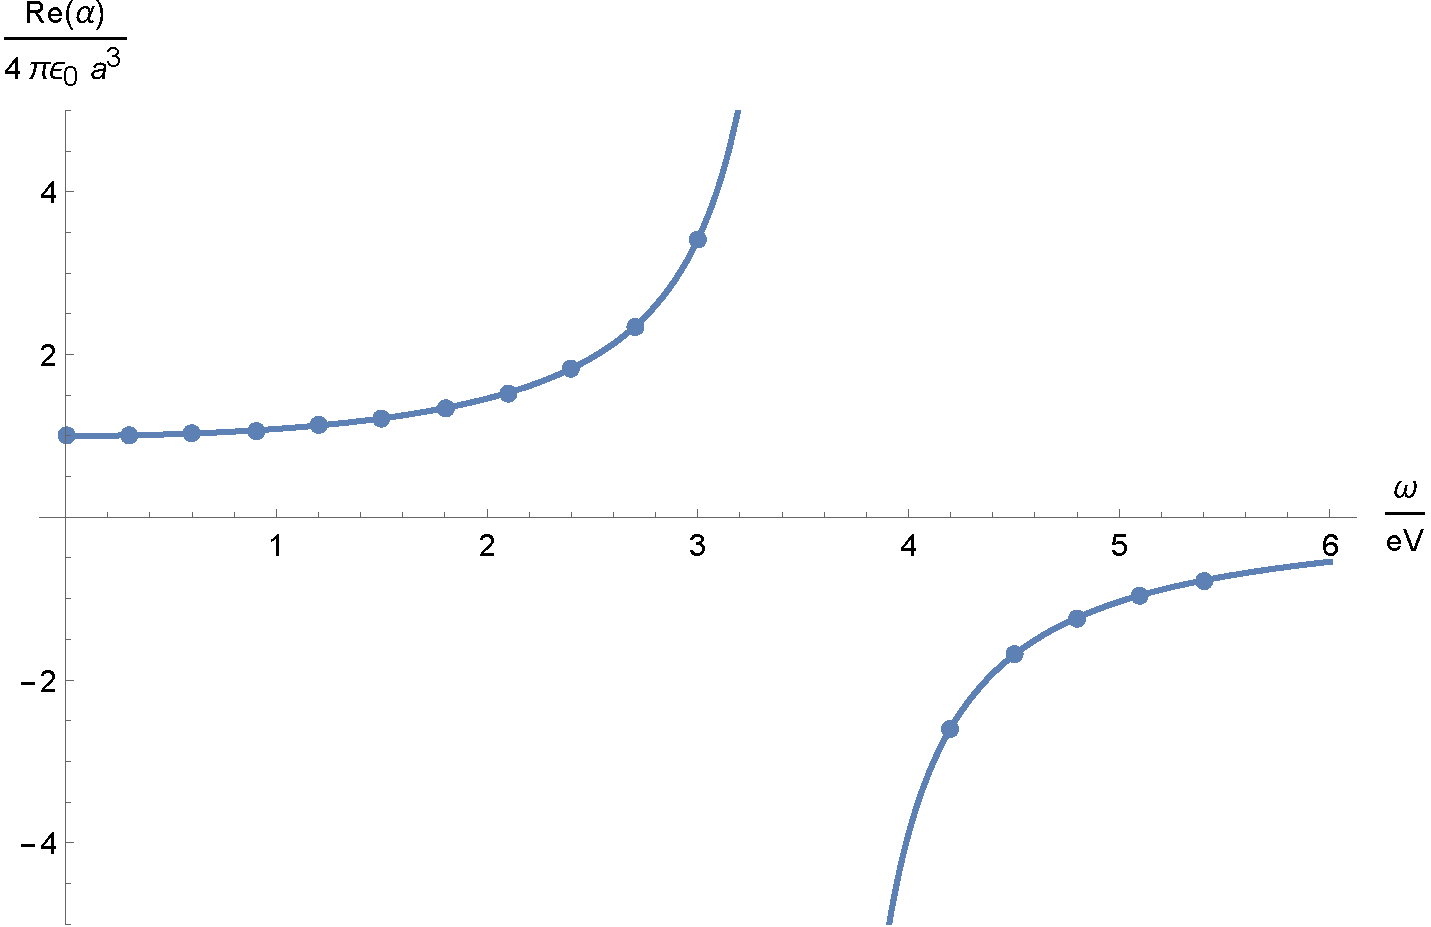
\includegraphics[width=\textwidth]{alpha-re.pdf}
    \end{subfigure}
    \begin{subfigure}{0.45\textwidth}
        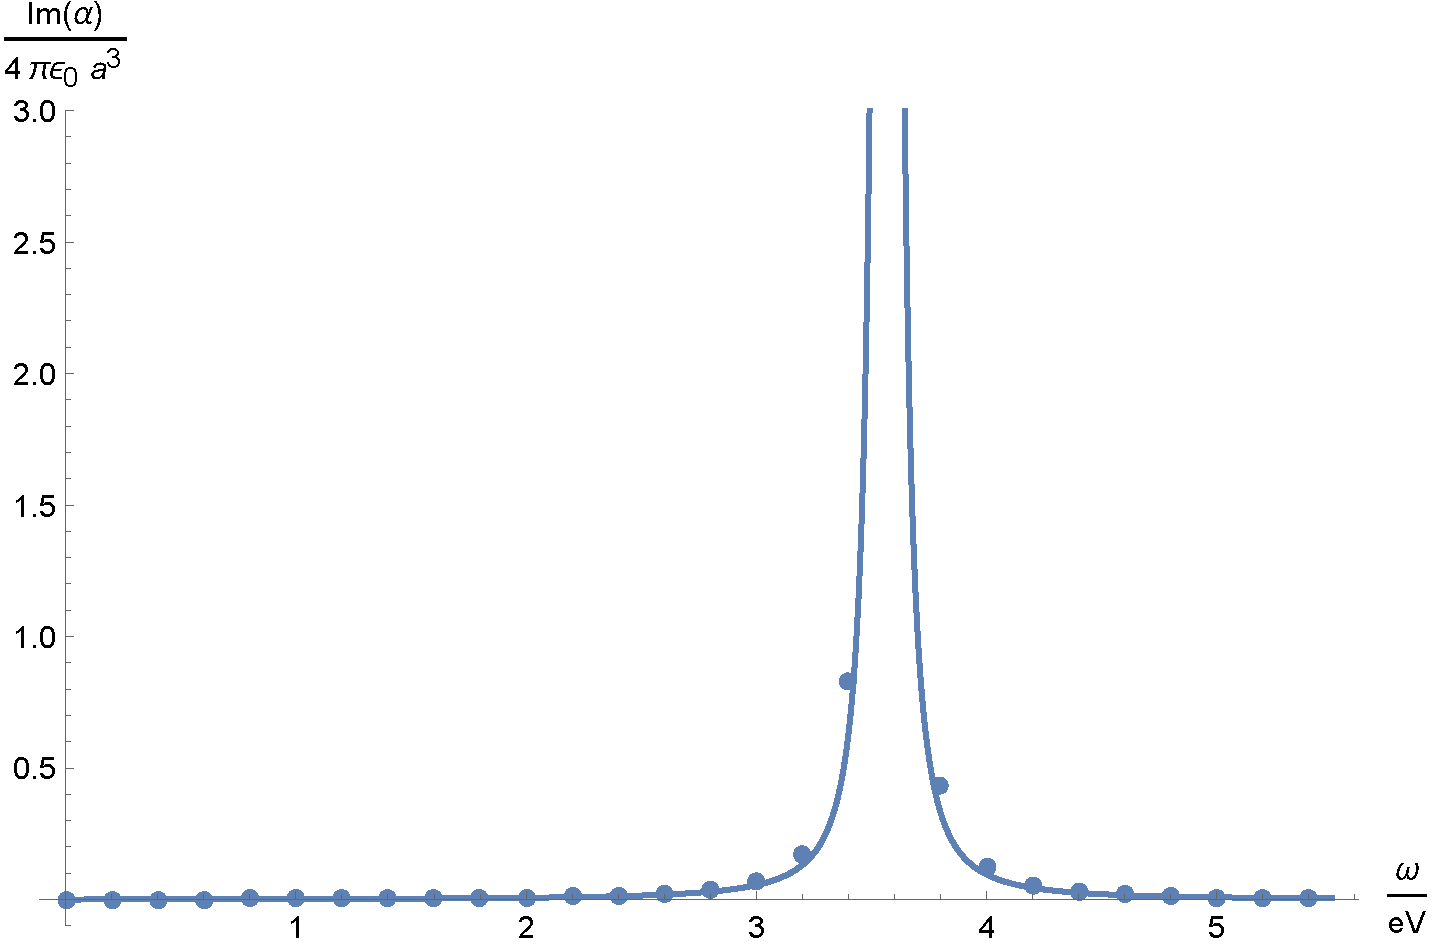
\includegraphics[width=\textwidth]{alpha-im.pdf}
    \end{subfigure}
    \caption{The real and the imaginary part of $\alpha(\omega)$. The lines are plotted by definition, and the scattered points are obtained by K-K relations. (a) The real part. (b) The imaginary part.}
    \label{fig:plot}
\end{figure}

\paragraph{Problem 1} Consider a one dimensional infinite chain on the $z$ direction consisting of metallic balls, 
each of which have radius $a$ and is made of a metal with permittivity
\begin{equation}
    \epsilon_\text{r} = 1 - \frac{\omega_\text{p}^2}{\omega (\omega + \ii \gamma)}.
\end{equation} 
When $a \to 0$, we have
\begin{equation}
    \alpha(\omega) = 4 \pi \epsilon_0 a^3 \frac{\epsilon_\text{r}(\omega) - 1}{\epsilon_\text{r}(\omega) + 2},
\end{equation}
We use Mathematica to plot the real and the imaginary part of $\alpha(\omega)$ in \prettyref{fig:plot}. 
TODO: features

\paragraph{}

\paragraph{Problem 2} We need to solve 
\begin{equation}
    \vb*{p}_m = \alpha (\vb*{E}_\text{ext}(\vb*{r}_m) + \omega^2 \mu_0 \sum_{n \neq m} \tensor{\vb*{G}}(\vb*{r}_m - \vb*{r}_n) \cdot \vb*{p}_n),
\end{equation}
and when there is no external field, by the Bloch condition 
\begin{equation}
    \vb*{p}_m = \vb*{u} \ee^{\ii k z_m},
\end{equation}
we have 
\[
    \vb*{u} \ee^{\ii k z_m} = \alpha \omega^2 \mu_0 \sum_{n \neq m} \tensor{\vb*{G}}(\vb*{r}_m - \vb*{r}_n) \cdot \vb*{u} \ee^{\ii k z_n},
\]
\[
    \left( \tensor{\vb*{I}} - \alpha \omega^2 \mu_0 \sum_{n \neq m} \tensor{\vb*{G}}(\vb*{r}_m - \vb*{r}_n) \ee^{\ii k z_n} \ee^{- \ii k z_m}  \right) \vb*{u}  = 0,
\]
and we have 
\begin{equation}
    \tensor{\vb*{M}} = \alpha^{-1} \tensor{ \vb*{I}} - \omega^2 \mu_0 \sum_{n \neq m} \tensor{\vb*{G}}(\vb*{r}_m - \vb*{r}_n) \ee^{\ii k (z_n - z_m)}, \quad \tensor{\vb*{M}} \vb*{u} = 0,
    \label{eq:eigen-problem}
\end{equation}
and we need to evaluate 
\begin{equation}
    \tensor{\vb*{W}} = \omega^2 \mu_0 \sum_{n \neq m} \tensor{\vb*{G}}(\vb*{r}_m - \vb*{r}_n) \ee^{\ii k (z_n - z_m)}.
\end{equation}

The dyadic Green function is 


The eigenvalues are actually ``eigen polarization'':
\begin{equation}
    \tensor{\vb*{M}} \cdot \vb*{u} = \frac{1}{\lambda^\text{eigen}} \vb*{u}.
\end{equation}

In the $\gamma \to 0$ limit, \eqref{eq:eigen-problem} can be written as 
\begin{equation}
    H \psi = \frac{\omega^2}{\omega_\text{p}^2} \psi,
\end{equation}
where 


\end{document}